\section*{Introducción}

En este artículo de final de año vamos a dar cierre al curso de Octave
que os hemos dado a lo largo de este primer volumen de la revista con
una series de problemas que podemos resolver con \emph{Octave}. Espero
leáis los problemas y antes de mirar la solución os déis un tiempo
para hacerlo por vosotros mismos. Es maravilloso encontrar la solución
por uno mismo.

Durante el año hemos dado unas nociones básicas de \emph{Octave} y
puedes aumentar los conocimientos usando, por ejemplo, el siguiente
tutorial
\url{http://en.wikibooks.org/wiki/Octave_Programming_Tutorial}.

\section{Esperanza de vida}
 
Según la organizacion mundial de la salud la definición de esperanza
de vida es como sigue: años que un recién nacido puede esperar vivir
si los patrones de mortalidad por edades imperantes en el momento de
su nacimiento siguieran siendo los mismos a lo largo de toda su
vida. Hacer un cálculo de esta cantidas es muy complicado y se tiene
en cuenta factores como por ejemplo la medicina, la higiene, las
guerras, etc.

Lo que os proponemos es lo siguiente: dado la esperanza de vida de
Ángola proporcionada por el banco mundial de datos
(\url{http://datos.bancomundial.org/}) que tenemos datos desde 1980 a
2012, os proponemos resolváis el desafío A.

\begin{mybox}
  \cappar A: ¿En qué año tiene previsto el pueblo angolano tener una
  esperana de vida de 80 años?\vspace{1.5cm}
\end{mybox}



\vspace{1cm} 
\textcolor{blue}{\Large Nuestra Solución}\\ 
Hemos coleccionado los datos
en un archivo \emph{Hopelife.csv}. Los vamos a cargar a Octave y vamos
a echarle un vistazo a estos. El código lo podrás visualizar en la
sección de códigos de la revista en \url{www.revistasolucoes.com}.
\begin{table}
\begin{center}
\begin{tabular}{cc}
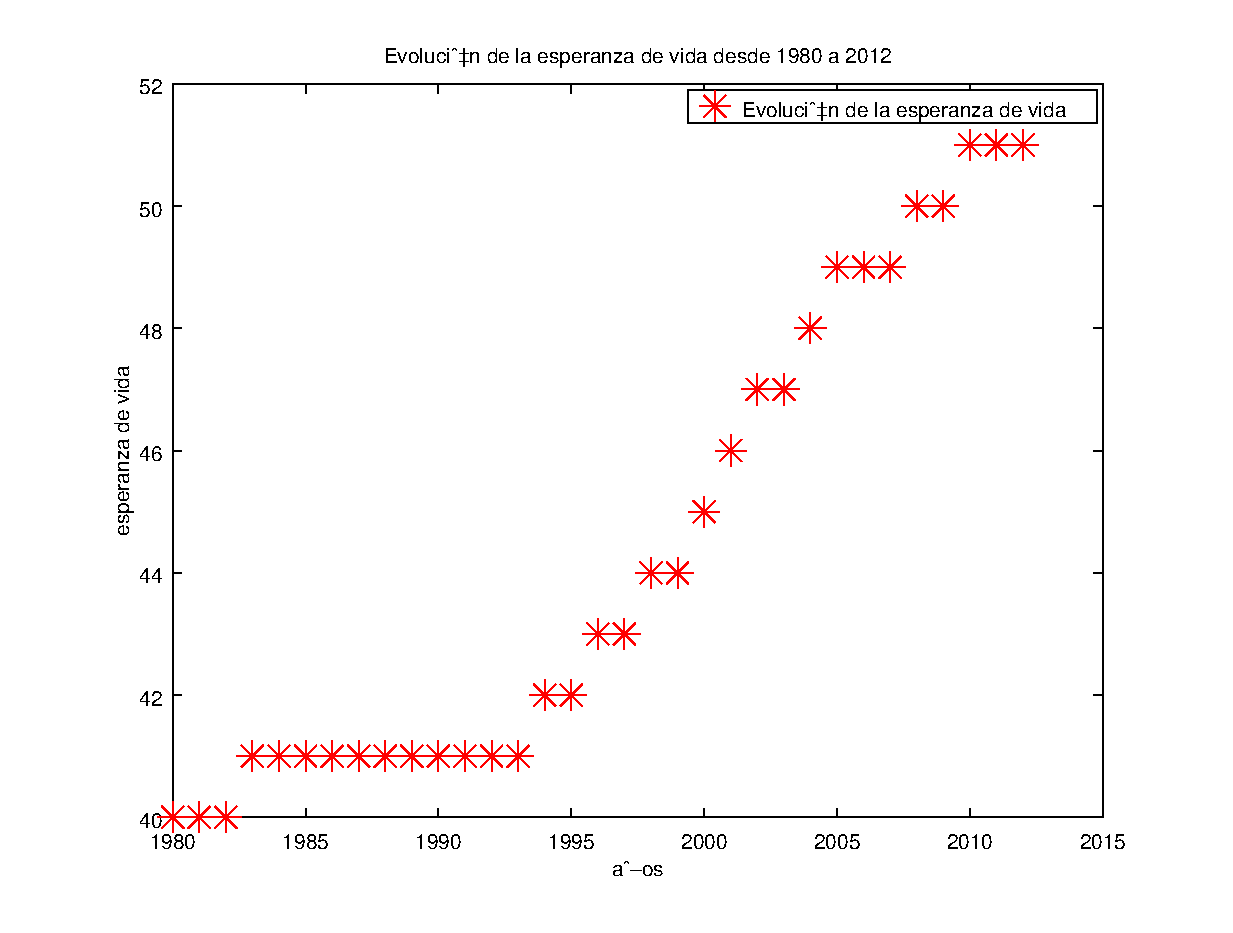
\includegraphics[scale=.45]{DatosPuros.eps} & 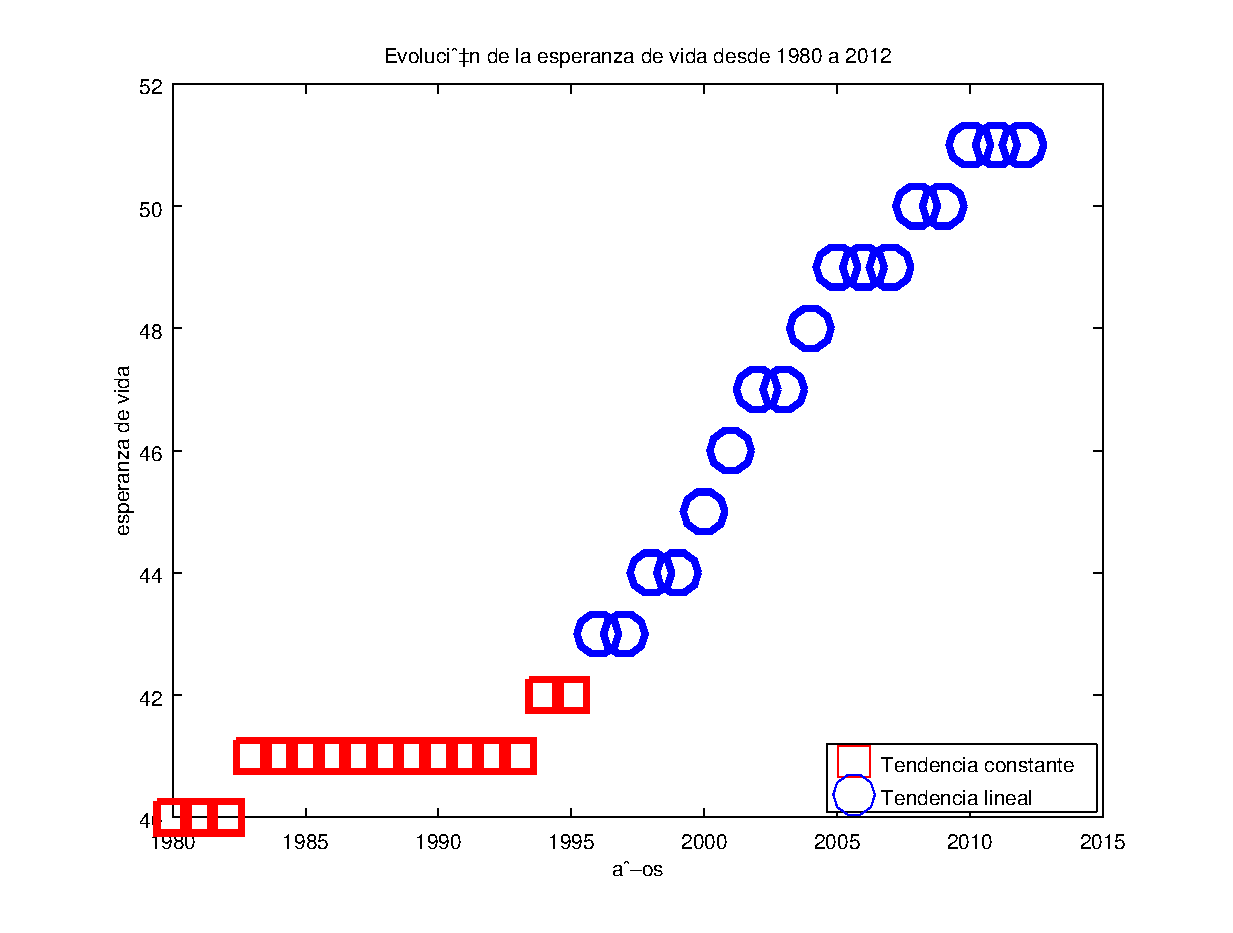
\includegraphics[scale=.45]{DatosTendencia.eps}\\
(A) & (B) \\
\end{tabular}\caption{(A): Evolución esperanza de vida desde 1980 a 2012, (B):Clusterización de los datos }
\end{center}
\end{table}\label{datos}



Si observamos la Tabla \ref{datos}, gráfico (A) tenemos claramente dos
tendencias en los datos. Una tendencia constante y una tendencia
lineal. Ambas las mostramos en el gráfico:

Y si vamos a la historia de Ángola, la tendencia constante corresponde
con años de la guerra civil. Esta terminó en 2002 pero vamos a
quedarnos con los datos desde el año 1996 ya que parece están en la
misma tendencia que de los años posteriores.

La idea de lo que vamos a hacer es lo siguiente: nuestro objetivo es
buscar una funcion $f(n)$ que nos da la esperanza de vida en el año
$n$. Como hemos dicho antes la tendencia que parecen tener los datos
(recuerda que nos hemos quedado con los datos azules en la Tabla
\ref{datos}, gráfico (B)) es una tendencia lineal. Existe un concepto en
estadísticaue nos asegura que nuestra intuición está en lo correcto y
es el \emph{coeficiente de correlación} o \emph{coeficiente de
  correlación lineal de Pearson}. Este coeficiente que denotaremos por
$\rho$ mide el grado de covariación entre dos distintas variables
relacionadas linealmente, denotémolas $x$ e $y$. El cálculo del
coeficiente de correlación entre dos variables $x$ e $y$ es sencillo y
viene dado por la fórmula $\rho=\frac{\sigma_x \sigma_y}{\sigma_{xy}}$
donde $\sigma_x$ o $\sigma_y$ son las desviaciones típicas de las
variables $x$ e $y$ respectivamente y $\sigma_{xy}$ la covarianza
entre las dos variables. El parámetro $\rho$ cumple que su rango de
valores está entre $-1$ y $1$ y lo podemos interpretar como sigue:
\begin{itemize}
\item Si $\rho \sim 1$ significa correlación lineal positiva.
\item Si $\rho \sim -1$ significa correlación lineal negativa.
\item Si $\rho \sim 0$ significa que las variables no tienen correlación lineal.
\end{itemize}

En \emph{Octave} existe el comando \emph{cor} que calcula la
correlación entre dos variables:
\begin{octavebox}
  \begin{verbatim}
x=datos(17:end,1);
y=datos(17:end,2);
disp('El coeficiente de correlación')
cor(x,y)
\end{verbatim}
\end{octavebox}
Y el resultado que se obtiene es de $0.98473$ por tanto nuestra
intuición queda apoyada por este concepto matemático y tiene mucho
sentido realizar una regresión lineal. Esto es buscar una función
$f(n)=\theta_1+\theta_2 \cdot n$ para la previsión de la esperanza de
vida en el año $n$.  Existen varios métodos para calcular las
constantes $\theta_1$ y $\theta_2$ del modelo. No vamos a dar muchos
detalles de ello, puedes buscarlo en cualquier libro de estadística
pero te diremos que un método rápido que se puede usar para bases de
datos pequeñas es el método de las ecuaciones normales que nos dan la
solución directamentre de la siguiente fórmula:
\begin{equation}
\theta=\left[
\begin{array}{c}
\theta_1\\
\theta_2\\
\end{array}
\right]=inv(X^t \cdot X)\cdot X^t \cdot y
\end{equation}
donde $X=\left[
\begin{array}{cc}
1 & \vdots\\
\vdots & x\\
1 & \vdots\\
\end{array}
\right]$.

Si sigues las instrucciones puedes ver que la función resultante y que
predice la esperanza de vida en el año $n$ es $f(n)=-1067,5+0.55 \cdot n$.  Usando esta
gráfica podemos augurar que si el crecimiento de Ángola va en la
dirección que marca el pueblo angolano tendrá una esperanza de vida de
80 años para el año 2063.  Damos algunos resultados en la siguiente tabla:
\begin{table}
\begin{center}
\begin{tabular}{cc}
\hline
Año & Esperanza de vida\\
\hline
2030 & 62\\
2050 & 73\\
2063 & 80\\
\hline
\end{tabular}
\end{center}\caption{Algunas previsiones futuras sobre la esperanza de vida angolana}
\end{table}






%\vspace{3cm}
%\noindent
%\includegraphics[width=\textwidth]{pubmm2.png}

\newpage
%%% Local Variables: 
%%% mode: latex
%%% TeX-master: "informaticaeningenieria"
%%% End: 



